\documentclass{beamer}

\mode<presentation>
{
  \usetheme{Boadilla}
  \beamertemplatenavigationsymbolsempty
}
\setlength\abovecaptionskip{0pt}

\usepackage{fontspec}
\setmainfont{Liberation Serif}
\setsansfont{Liberation Sans}
\setmonofont{Liberation Mono}

\usepackage{polyglossia}
\setdefaultlanguage[variant=us]{english}

\usepackage{csquotes}
\usepackage{xcolor}

\title[Identifying Woodblocks]{Identifying Woodblocks from the Bukan Collection}
\subtitle{Progress Report: The Failure of pHashes}
\author{Thomas Leyh}
\institute[]{University of Freiburg, Germany}
\date{December 2nd, 2019}

\begin{document}
  \begin{frame}
    \titlepage
  \end{frame}

  \begin{frame}
    \frametitle{Reminder on pHashes}
    I tried to find pages that were printed with the same woodblock.

    \bigskip
    Using \alert{perceptual hashes} I looked for perceptually similar pages.

    \bigskip
    In total, I was comparing 90,000 x 90,000 images.
  \end{frame}

  \begin{frame}
    \frametitle{pHash Expectation}
    \begin{figure}
      \centering
      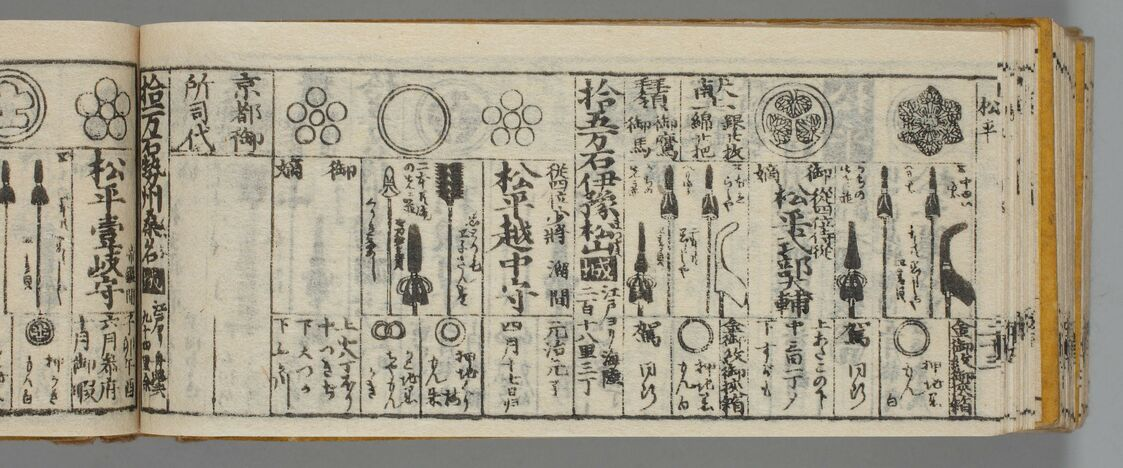
\includegraphics{200019552_00050}
      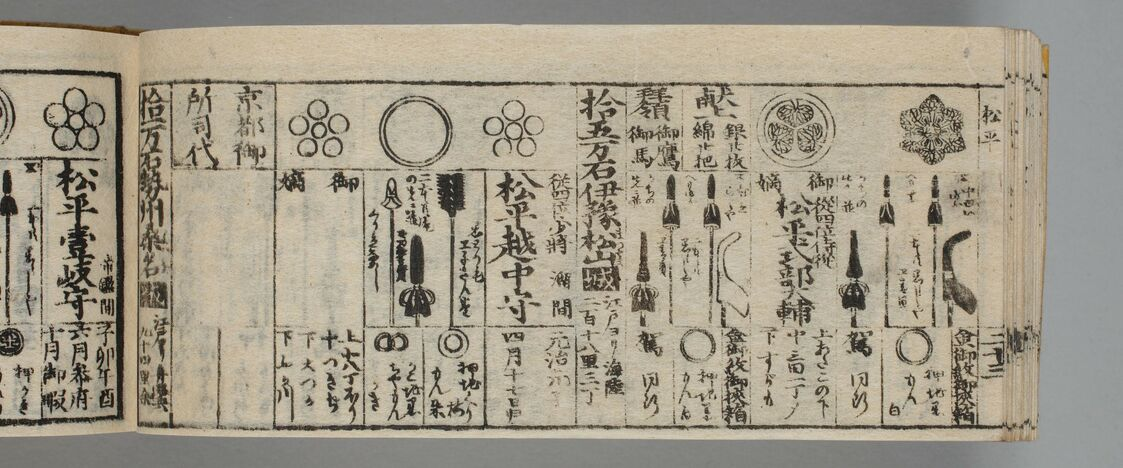
\includegraphics{200019556_00050}
    \end{figure}
  \end{frame}
  
  \begin{frame}
    \frametitle{pHash Reality}
    \begin{figure}
      \centering
      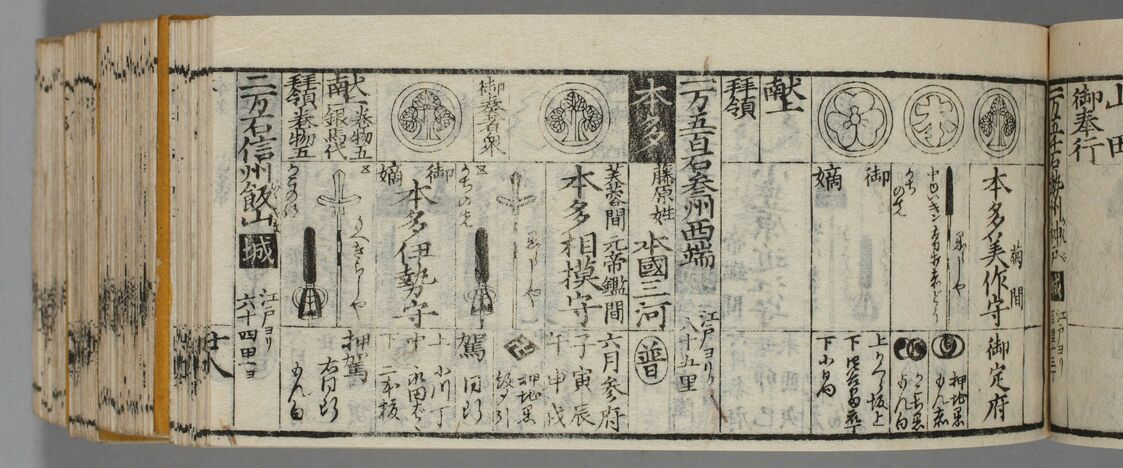
\includegraphics{200019601_00059}
      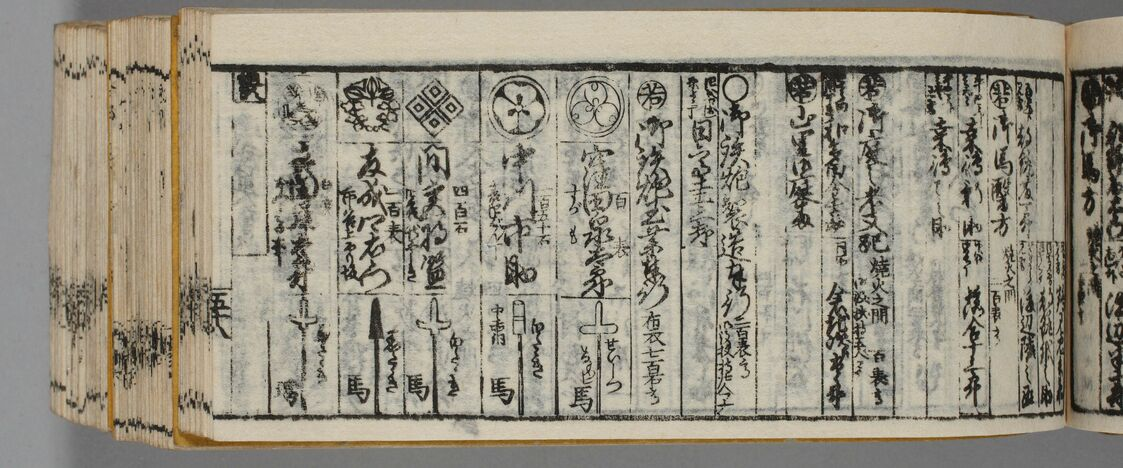
\includegraphics{200019602_00127}
    \end{figure}
  \end{frame}

  \begin{frame}
    \frametitle{An Attempted Explanation}
    pHashes:
    \begin{itemize}
      \item Are based on \emph{Discrete Cosine Transform} from signal processing
      \item Use image features
      \item Hence, not \alert{context-aware}
    \end{itemize}

    \bigskip
    
    It is really hard to quickly compare texts without looking at the content.
  \end{frame}
  
  \begin{frame}
    \frametitle{Back to explicit Feature Extraction}
    I started experimenting with \emph{OpenCV} algorithms,\\i.e. combinations of:
    \begin{itemize}
      \item Page Segmentation
      \item Page Binarization
      \item Feature Extraction and Matching
    \end{itemize}

    \bigskip
    For that reason, I prepared annotated test data…
  \end{frame}
  
  \begin{frame}
    \frametitle{Distribution of Bukan editions}
    \begin{figure}
      \centering
      \includegraphics[width=0.7\linewidth]{bukan-distribution}
      \caption{Books with more than two editions;
        \textcolor{orange}{orange} books are used for test and validation}
    \end{figure}
  \end{frame}

  \begin{frame}
    \frametitle{Annotation Results}
    \begin{itemize}
    \item Comparing 44 books of Shūchin Bukan
    \item Three woodblocks with multiple editions
      \begin{itemize}
        \item 12 editions
        \item 15 editions
        \item 17 editions
      \end{itemize}
      \item Around 155 pages per book
      \item 7,000 pages in total for playing around with
    \end{itemize}

    \bigskip
    I just need to pay attention not to overfit to Shūchin Bukan.
  \end{frame}

  \begin{frame}
    \frametitle{Next Step}
    Reproducing \emph{``Differential Image Reading''} on my test data.
  \end{frame}

\end{document}
% Local Variables:
% TeX-engine: xetex
% End:
